\documentclass[]{article}

% accenti
\usepackage[utf8]{inputenc}
% rimuove indentatura
\usepackage[parfill]{parskip}
% colori
\usepackage{color}
% per cambiare i margini della pagina
\usepackage{vmargin}
% per fissare le figure
\usepackage{float}

\usepackage{graphicx}
\begin{document}

\title{ABR vs ARN}
\author{Federico Magnolfi}
\date{May 18, 2017}
\maketitle

\section{Introduzione}
Si vogliono analizzare le differenze tra Alberi Binari di Ricerca e Alberi Rosso-Neri. Si scriverà un programma che permetta di capire vantaggi e svantaggi di queste due strutture dati.

\section{Descrizione}
Un albero è una struttura dati composta da nodi: ogni nodo contiene una chiave, eventualmente altri valori, ed ha una lista di nodi figli. Esiste un nodo particolare detto root (radice) dal quale discendono tutti gli altri nodi; un nodo senza figli è detto foglia. Si dice cammino tra due nodi una sequenza di nodi che li unisce, la lunghezza del cammino è data dal numero di nodi che si incontrano nel cammino, escluso il primo. La lunghezza del cammino che inizia e finisce nello stesso nodo è quindi 0; si dice altezza $h$ dell'albero la lunghezza massima tra i cammini che uniscono la radice alla foglie.

Si parla di albero binario quando ogni nodo ha al massimo due figli: si indicano come figlio sinistro e destro.

Un Albero Binario di Ricerca è un albero binario dove i nodi sono organizzati con il seguente criterio: tutti i discendenti sinistri di un nodo hanno chiave minore o uguale del nodo antenato, per i discendenti destri la chiave è maggiore o uguale.

Negli Alberi Binari di Ricerca, il bilanciamento dell'albero dipende dall'ordine di inserimento dei nodi: se i nodi vengono inseriti in ordine di chiave crescente (o decrescente), l'albero sarà completamente sbilanciato, ovvero ogni nodo esclusa la foglia avrà soltanto il figlio destro (o sinistro). L'albero è perfettamente bilanciato quando ogni nodo, escluse le foglie, ha esattamente due figli.

Gli Alberi Rosso-Neri sono particolari Alberi Binari di Ricerca che riescono a mantenersi piuttosto bilanciati. Riescono a farlo attribuendo un colore al nodo e modificando opportunamente le operazioni di inserimento e cancellazione. Un albero Rosso-Nero soddisfa le seguenti proprietà:
\begin{itemize}
\item[1)] Ogni nodo è rosso o nero
\item[2)] La radice è nera
\item[3)] Ogni foglia è nera
\item[4)] Se un nodo è rosso, allora entrambi i figli sono neri
\item[5)] Tutti i cammini da ogni nodo alle foglie contengono lo stesso numero di nodi neri
\end{itemize}

L'altezza nera di un nodo è il numero di nodi neri che si incontrano lungo il cammino tra il nodo (escluso) e una qualsiasi foglia (inclusa): è uguale per ogni cammino per la proprietà 5.
Per la proprietà 4, ogni nodo ha un'altezza nera che è maggiore o uguale della metà dell'altezza del nodo.

\section{Analisi teorica}
Su queste due strutture dati, le operazioni di inserimento, ricerca e cancellazione, avranno un costo massimo proporzionale all'altezza dell'albero, $O(h)$.

Per l'Albero Binario di Ricerca (ABR), nel caso in cui i dati vengono inseriti in ordine, si ha $h = n-1$, quindi per ogni operazione il costo massimo è $O(n)$. 
Per alcune permutazioni dell'ordine degli inserimenti, l'albero viene perfettamente bilanciato e $h = O(lg(n))$. L'altezza è proporzionale al logaritmo del numero di nodi, anche se gli inserimenti vengono fatti in ordine casuale, solo che ci saranno costanti con valori più grandi del caso precedente.

Per gli Alberi Rosso-Neri (ARN), grazie alle proprietà viste precedentemente, per ogni ordine di inserimento si ha $h = O(lg(n))$.

Visto che il costo di un singolo inserimento è $O(h))$, il costo di $n$ inserimenti sarà $O(n*h))$, ovvero $O(n^2)$ oppure $O(n lg(n))$ a seconda del caso.

\section{Descrizione esperimenti}
Si eseguono i test all'aumentare di $n$. I valori di $n$ da testare sono contenuti all'interno di un array: per ognuno di essi, sia per ABR che per ARN, si esegue l'inserimento di $n$ numeri ordinati, di $n$ numeri in ordine casuale e di $n$ numeri nell'ordine di quelli che saranno i livelli di ABR. Nei vari casi si misurano i tempi di inserimento e l'altezza dell'albero.

Si sarebbe potuto misurare anche i tempi di ricerca, ma essi sarebbero stati simili ai tempi di inserimento, soltanto con costanti più piccole.

I valori di $n$ testati sono i seguenti:

[0, 100, 200, 400, 600, 800, 1000, 1500, 2000, 3000, 4000, 5000, 6000, 7000].

\subsection*{Piattaforma di test}
Il test viene eseguito su un computer desktop con le seguenti caratteristiche:
\begin{itemize}
\item Sistema Operativo: Linux Mint 18.1
\item CPU: Intel Core i5-2400 (6 MB cache, 3.40 Ghz)
\item RAM: 16 GB
\item linguaggio di programmazione e interprete: Python 3.5
\item IDE: PyCharm 2017
\end{itemize}

\section{Documentazione del codice}
Il programma è composto da 4 file: abr.py, arn.py, test.py, exp.py.

\subsection*{abr.py}
Implementa la classe Node e la classe ABR.
La classe Node contiene i seguenti attributi:
\begin{itemize}
\item key: chiave del nodo
\item left: nodo figlio sinistro
\item right: nodo figlio destro
\item father: nodo padre
\end{itemize}
La classe ABR ha un attributo root che tiene traccia del nodo radice. I metodi implementati utili fini dell'esperimento sono i seguenti:
\begin{itemize}
\item insert(key): inserisce un nodo con chiave key nell'albero. L'inserimento viene fatto in modo iterativo in quanto più efficiente della versione ricorsiva.
\item height(): restituisce l'altezza dell'albero
\end{itemize}

\subsection*{arn.py}
Implementa la classe ColoredNode e la classe ARN.
La classe ColoredNode contiene i seguenti attributi:
\begin{itemize}
\item key: chiave del nodo
\item left: nodo figlio sinistro
\item right: nodo figlio destro
\item father: nodo padre
\item isBlack: booleano che indica se il nodo è nero (True) o rosso (False)
\end{itemize}
La classe ARN ha un attributo root che tiene traccia del nodo radice, e un attributo NIL che è il nodo con chiave nulla usato come sentinella. I metodi implementati utili fini dell'esperimento sono i seguenti:
\begin{itemize}
\item insert(key): inserisce un nodo con chiave key di colore rosso nell'albero, richiamando poi il metodo fixup passandogli il nodo inserito.
\item fixup(z): controlla se il nodo z rispetta le proprietà dell'albero, se così non fosse chiama metodi per mantenere la validità di esse.
\item height(): restituisce l'altezza dell'albero
\end{itemize}

\subsection*{test.py}
Contiene tre funzioni:
\begin{itemize}
\item bestOrder(orderedArray): dato un array ordinato in ingresso, restituisce un array opportunamente permutato che indichi l'ordine degli inserimenti da fare per avere il caso migliore.
\item test(array): dato un array qualsiasi, inserisce gli elementi dell'array (nell'ordine in cui si trovano) in un nuovo ABR ed in un nuovo ARN, misurando e ritornando i tempi di inserimento e le altezze.
\item runAllTests(numbers): data una lista di valori di $n$ da testare, per ogni $n$ esegue il test nel caso ordinato, migliore e random. Per il random viene fatta la media su 10 test. I risultati dei test vengono salvati in una lista, che alla fine viene ritornata dalla funzione.
\end{itemize}
La lista contenente gli esiti dei test contiene un elemento del seguente tipo per ogni valore di $n$:
\begin{verbatim}
[n, ordABR_H, ordARN_H, bestABR_H, bestARN_H, randABR_H, randARN_H,
ordABR_T, ordARN_T, bestABR_T, bestARN_T, randABR_T, randARN_T]
\end{verbatim}
Nei nomi delle variabili, ord/best/rand indica l'ordine di inserimento, ABR/ARN indica il tipo di struttura dati, H/T indica altezza o tempo.

\subsection*{exp.py}
Chiama la funzione runAllTests situata in test.py passandogli la lista degli $n$ da testare.

Analizza l'esito del test costruendo due grafici, uno per le altezze e uno per i tempi di inserimento. In entrambi i grafici, la funzione relativa all'inserimento ordinato in ABR viene mostrata con una scala per l'asse y diversa, in quanto molto più grande rispetto alle altre, l'asse x è condiviso.

\section{Risultati sperimentali}
Si ricorda che lista contenente gli esiti dei test contiene un elemento del seguente tipo per ogni valore di $n$:
\begin{verbatim}
[n, ordABR_H, ordARN_H, bestABR_H, bestARN_H, randABR_H, randARN_H,
ordABR_T, ordARN_T, bestABR_T, bestARN_T, randABR_T, randARN_T]
\end{verbatim}

L'output del programma è il seguente:
\begin{verbatim}
[0, 0, 0, 0, 0, 0.0, 0.0, 0.0, 0.0, 0.0, 0.0, 0.0, 0.0]
[100, 99, 10, 6, 6, 12.4, 7.2, 0.0007, 0.0006, 0.0002, 0.0003, 0.0002, 0.0004]
[200, 199, 12, 7, 7, 14.8, 8.4, 0.0027, 0.0013, 0.0004, 0.0007, 0.0005, 0.0009]
[400, 399, 14, 8, 8, 17.6, 9.8, 0.01, 0.0028, 0.0008, 0.0015, 0.0011, 0.0019]
[600, 599, 15, 9, 9, 18.8, 10.5, 0.0221, 0.0054, 0.0012, 0.0023, 0.0015, 0.0031]
[800, 799, 16, 9, 9, 19.7, 10.9, 0.039, 0.0059, 0.0017, 0.0039, 0.002, 0.0056]
[1000, 999, 16, 9, 9, 20.7, 11.0, 0.061, 0.0075, 0.002, 0.0043, 0.0028, 0.0051]
[1500, 1499, 17, 10, 10, 22.2, 12.0, 0.1373, 0.0117, 0.0033, 0.0067, 0.0042, 0.0098]
[2000, 1999, 18, 10, 10, 24.3, 12.5, 0.2429, 0.0167, 0.0046, 0.0081, 0.0055, 0.0137]
[3000, 2999, 19, 11, 11, 25.7, 13.0, 0.5423, 0.0248, 0.0066, 0.013, 0.0088, 0.0231]
[4000, 3999, 20, 11, 11, 26.5, 13.8, 0.9544, 0.0335, 0.0092, 0.0168, 0.016, 0.0264]
[5000, 4999, 21, 12, 12, 26.1, 14.1, 1.4746, 0.042, 0.0118, 0.0224, 0.0185, 0.0321]
[6000, 5999, 21, 12, 12, 27.6, 14.1, 2.1693, 0.0517, 0.0147, 0.0261, 0.0181, 0.0463]
[7000, 6999, 22, 12, 12, 27.9, 14.9, 2.8899, 0.0611, 0.017, 0.0313, 0.0262, 0.0475]
\end{verbatim}

I grafici di altezze (Figura \ref{graficoAltezze}) e tempi di inserimento (Figura \ref{graficoTempi}) relativi all'esperimento effettuato sono i seguenti:

\begin{figure}[H]
	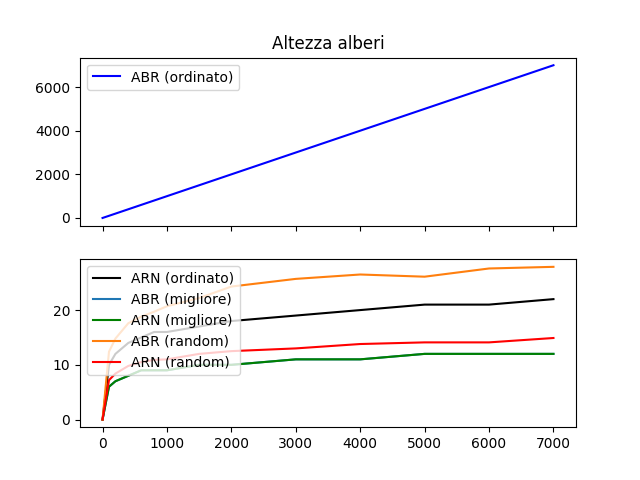
\includegraphics{altezze.png}
	\caption{Altezze degli alberi in funzione del numero di elementi}
	\label{graficoAltezze}
\end{figure}

\begin{figure}[H]
	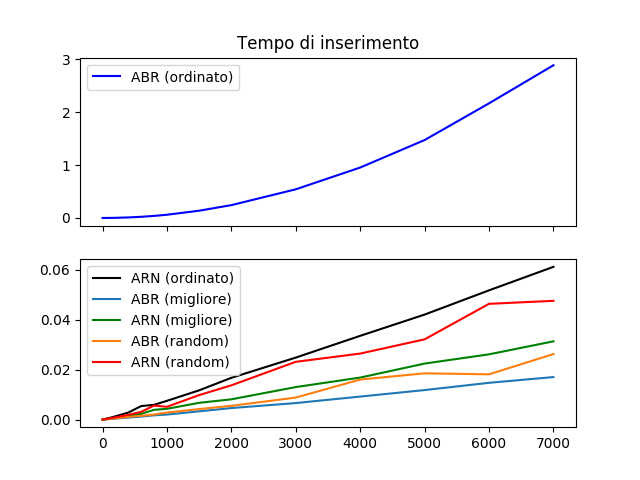
\includegraphics{tempi.png}
	\caption{Tempi di inserimento negli alberi in funzione del numero di elementi}
	\label{graficoTempi}
\end{figure}


\section{Analisi dei risultati}
Analizzando le altezze degli alberi nei vari casi, esse risultano sempre logaritmiche (con costanti diverse) con eccezione dell'altezza di ABR con inserimento ordinato che è lineare.
Nel caso migliore, le altezze di ABR e ARN sono minime e coincidono, negli altri casi invece ARN è sempre meglio di ABR, inoltre anche per ARN l'inserimento random produce sempre altezze minori dell'inserimento in ordine.

Analizzando i tempi di inserimento, essi stanno tutti in $O(n lg(n))$ (con costanti diverse), con l'eccezione di ABR con inserimento ordinato che sta in $O(n^2)$.
I tempi di ABR nel caso migliore e random sono leggermente migliori dei tre casi di ARN, mentre il tempo di inserimento ordinato in ABR è molto più grande di tutti gli altri casi.

\section{Conclusioni}
Gli esiti dell'esperimento sono compatibili con ciò che era stato previsto.

Si ritiene quindi che la struttura dati Albero Rosso-Nero sia preferibile al semplice Albero Binario di Ricerca, in quanto garantisce ottime prestazioni in ogni caso.


\end{document}